\documentclass[10pt,a4paper]{article}
\usepackage[margin=24mm]{geometry}
\usepackage[T1]{fontenc}
\usepackage{lmodern,microtype,amsmath,amssymb,mathtools}
\usepackage{graphicx,booktabs,longtable,array,xcolor,listings,tikz}
\usepackage{placeins}
\usetikzlibrary{arrows.meta,positioning}
\usepackage[hidelinks]{hyperref}
\hypersetup{pdftitle={Shared Cost Bags for Effectful E-Graph Extraction},pdfsubject={A whole-suite study on pristine eggcc}}
\renewcommand{\topfraction}{0.9}
\renewcommand{\textfraction}{0.08}
\usepackage{fancyhdr}
\definecolor{inkblue}{HTML}{205D85}
\definecolor{inkgreen}{HTML}{29744A}
\definecolor{lightblue}{HTML}{EAF2F8}
\definecolor{inkred}{HTML}{A33A3A}
\pagestyle{fancy}\fancyhf{}
\fancyhead[L]{\small Shared Cost Bags in Tiger}\fancyhead[R]{\small Technical Report}
\fancyfoot[C]{\thepage}\setlength{\headheight}{14pt}
\setlength{\parskip}{4pt}\setlength{\parindent}{0pt}
\lstset{basicstyle=\small\ttfamily,keywordstyle=\color{inkblue},
 commentstyle=\color{inkgreen},columns=fullflexible,keepspaces=true,
 frame=single,rulecolor=\color{black!20},breaklines=true,showstringspaces=false}
\newcommand{\tool}[1]{\texttt{#1}}
\newcommand{\mm}{\operatorname{minmerge}}
\title{\textbf{Shared Cost Bags for Effectful E-Graph Extraction}\\[4pt]
\large A Whole-Suite Study on Pristine eggcc}
\author{}\date{24 October 2026}
\begin{document}
\maketitle\vspace{-2em}
\begin{abstract}
Tiger's extractor accounts for DAG sharing by carrying a map of contributions
already paid for. We evaluate a representation-only optimization: copies share
an immutable sorted vector, while accumulation preserves the original per-key
minimum and unsigned arithmetic. Copying a bag becomes constant-time, although
individual merges need not become asymptotically cheaper. The evaluation covers
all 96 passing programs in a pinned, unmodified eggcc checkout and its locked
egglog dependencies. Each program follows the production three-pass pipeline;
independent paired extractions use identical captured graphs and require complete
output equality and a native cost/pick oracle.
\IfFileExists{abstract-results.tex}{All 96 programs and 288 pass snapshots satisfy the extraction gates. The geometric-mean cost-estimation ratio is 3.82$\times$; whole-extractor time improves by 1.052$\times$ geometrically and 1.104$\times$ in aggregate. The measured pipeline ratio is 0.995$\times$ geometrically, so this experiment does not demonstrate a pipeline-level speedup.
}{}
The report separates cost-estimation gains, whole-extractor performance, and
observed pipeline timing. It makes no GPU inference or global-optimality claim.
\end{abstract}

\section{Problem and scope}
Effectful extraction must select compatible operations, preserve state ordering,
and retain useful DAG sharing. Tiger combines global greedy cost estimation,
Statewalk dynamic programming, and subsequent DAG extraction \cite{eggcc}.
This change targets only the representation used by the \emph{global cost
estimator}. The cost model, candidate traversal, queues, Statewalk implementation,
final pure extraction, and tie rules remain unchanged.

We evaluate eggcc revision \texttt{ae80f82a403c1209fb084b115ee89470c7e66d0e}.
Pristine means its tracked source and exact locked dependencies are unchanged:
\tool{egglog-experimental} revision \texttt{08771f9} selects egglog kernel
\texttt{ebba7bb} \cite{experimental,engine}. This is a versioned engine stack,
not a claim to use the newest egglog revision. Cell/GPU inference patches,
Analyze, Bake, and history tracing do not generate the benchmark graphs.

The optimization is extraction bookkeeping. It shares copies of a cost bag,
rather than consuming learned RipSatCell certificates or skipping inference
matches. Optional CPU/Metal cost-recipe modes in the prototype are disabled.

\section{Preserving the cost information}
If shared computation $t$ costs 3, $A$ adds 1, and $B$ adds 2, their separate
totals are 4 and 5, but producing both can cost $3+1+2=6$. Both implementations
already account for that sharing; this example does not describe a correctness
bug in the baseline.

A cost object is $(s,B)$, where $s$ is the estimate and
$B:\mathcal C\rightharpoonup\mathbb U_{64}$ maps e-class identifiers to
accounted contributions. Its own overhead need not be included in $B$.
Accumulating child $c$ with cost $(s_c,B_c)$ into $(s_p,B_p)$ computes
\begin{align}
 h_c &= s_c-\sum_{x\in\operatorname{dom}(B_c)}B_c(x),\\
 B'_p &= \mm(B_p,B_c,\{c\mapsto h_c\}),\\
 s'_p &= s_p+\sum_x B'_p(x)-\sum_x B_p(x).
 \label{eq:update}
\end{align}
Here $\mm$ retains the union of key domains and takes the smaller unsigned
contribution at each repeated key. All additions and subtractions use the
original modulo-$2^{64}$ arithmetic. Zero contributions, repeated operands,
e-class identity, and the all-ones infinity sentinel are preserved.

\subsection{From hash nodes to shared immutable vectors}
The original \tool{SCost} contains an \tool{unordered\_map<EClassId,Cost>}.
Ordinary C++ copies copy its entries, including when children enter pairs and
candidate costs are assigned. The candidate uses a scalar and
\tool{shared\_ptr<const CostBag>}. A bag contains sorted unique key/value entries
and their cached modulo sum. Copies share the vector; every accumulation
creates a new vector and leaves previously published bags unchanged.
Independently computed equal vectors remain separate allocations.

\begin{figure}[ht]
\centering
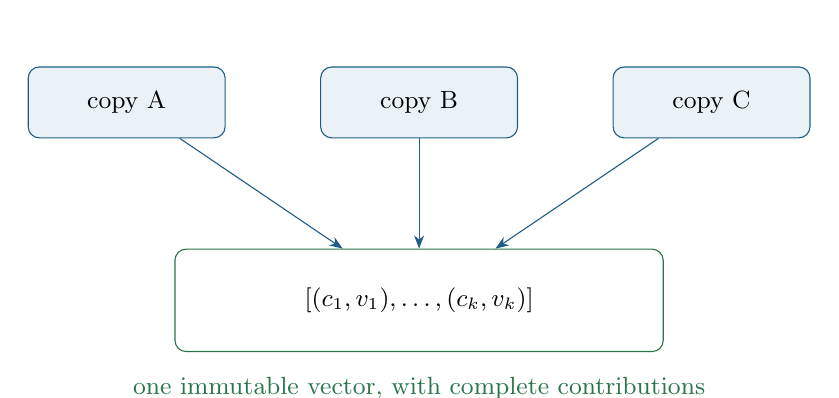
\begin{tikzpicture}[font=\small,>=Stealth,
 record/.style={draw=inkblue,rounded corners,fill=lightblue,minimum width=25mm,minimum height=9mm},
 bag/.style={draw=inkgreen,rounded corners,minimum width=62mm,minimum height=13mm}]
\node[record] (a) {copy A};
\node[record,right=12mm of a] (b) {copy B};
\node[record,right=12mm of b] (c) {copy C};
\node[bag,below=14mm of b] (s) {$[(c_1,v_1),\ldots,(c_k,v_k)]$};
\draw[->,inkblue] (a)--(s);\draw[->,inkblue] (b)--(s);\draw[->,inkblue] (c)--(s);
\node[below=2mm of s,text=inkgreen] {one immutable vector, with complete contributions};
\end{tikzpicture}
\caption{Cost-object copies share storage. Accumulation creates a new bag.
These are bookkeeping objects, not e-graph partitions.}
\end{figure}

\begin{lstlisting}[caption={Representation-level accumulation (schematic).}]
overhead = child.sum - child.bag.total
next = merge_sorted_min(parent.bag.entries, child.bag.entries)
insert_or_min(next, child_class, overhead)
total = sum_mod_u64(next)
parent.sum += total - parent.bag.total
parent.bag = immutable(next, total)
\end{lstlisting}

\subsection{Preservation argument}
Assume the vector and the original map contain the same key/value pairs, and the
cached total equals their modulo sum. Copying preserves this invariant.
Ordered merging and the child-key insertion compute the same domain and
pointwise minima as hash-map updates. The cached child sum yields the same
overhead; Equation~\ref{eq:update} changes the parent estimate by the same
contribution difference. Thus accumulation preserves the map and estimate.

Induction over the unchanged traversal gives identical estimates and comparisons
for the same ordered input. The implementation instantiates the same greedy body
with either representation. A separate oracle checks its cost and pick vectors,
and complete output equality checks the downstream extractor on observed inputs.
This preserves the baseline's heuristic decisions; it does not prove global
optimality.

\section{Complexity and the tradeoff}
For a copied bag of size $k$, an accumulator of size $m$, and a child bag of
size $n$, the relevant costs are:
\begin{center}
\begin{tabular}{lll}
\toprule
Operation & Original hash bag & Shared sorted bag\\
\midrule
Copy a cost object & $\Theta(k)$ & $O(1)$ reference copy\\
Accumulate one child & expected $O(n+1)$ & $O(m+n+1)$\\
Read child contribution sum & $O(n)$ scan & $O(1)$ cached total\\
Materialized storage & nodes and buckets & contiguous pairs\\
\bottomrule
\end{tabular}
\end{center}
The vector merge also visits the accumulator. Therefore it is incorrect to claim
that every merge becomes asymptotically faster. Saved deep copies and allocations
must outweigh this extra sequential work. Small operator arities can limit prefix
merges, but that is a workload property. Regressions are retained in the study.
Logical entry counts are work counters, not measurements of resident memory.

Parsing, region construction, Statewalk search, final extraction, and output
remain. If an accelerated phase occupies fraction $f$ and improves by factor $r$,
the explanatory Amdahl expression is
\[
 S=\frac{1}{(1-f)+f/r}.
\]
A large phase gain can therefore coexist with a small whole-process gain.
This equation is not substituted for measured pipeline performance.

\section{Experimental design}
\subsection{Inventory and clean builds}
The inventory is every \tool{.bril} and \tool{.rs} file under
\tool{benchmarks/passing}: 64 Bril, 30 PolyBench, one raytracer, and one
Fenwick-tree program. No case is selected by expected speedup.
A clean shallow checkout preserves the exact upstream commit. Remote Git
fetches timed out, so verified Git objects from a clean local mirror were
transferred; no existing eggcc binary was reused. Registry archives were checked
against the lockfile before seeding an isolated build cache. All executables
were rebuilt.

The runner rejects dirty upstream tracked sources and dirty Git dependencies.
It records revisions, lockfile/source/executable hashes, compiler, machine, and
affinity. The fresh Debian 12 container uses Rust 1.88.0, LLVM 18.1.8, and the same
C++ compiler/flags for both Tiger builds. Timed work is pinned to logical CPU 2,
a performance-core hardware thread of an Intel Core i7-13700KF. The container has
24 GiB memory and no swap allowance. These are CPU measurements.

\subsection{Production and frozen-graph comparisons}
\textbf{Production pipeline.}
Both lanes run the exact same pristine eggcc binary; only its sibling
\tool{tiger} executable changes. The original \tool{parallel} pass schedule and
single-threaded egglog configuration are retained. Each pass's extracted program
feeds the next pass. Both lanes use upstream \tool{--egraph-out-dir} and
\tool{--run-data-out}. Consequently, pipeline wall time includes graph capture;
it is not a CLI measurement without capture.

\textbf{Frozen graphs.}
Every native pass graph is replayed unchanged through original Tiger and shared
bags. These are the primary extraction measurements. A separate
timer-instrumented original-cost lane measures the targeted phase. A separate
oracle recomputes native costs and picks. Neither extra lane contributes to
the primary whole-extractor speedup. The candidate's existing lightweight timers
and counters remain enabled and are charged to its measured time.

\subsection{Gates, ordering, and failures}
A frozen-graph ratio requires successful processes, byte-identical complete
selected-program outputs, and a passing native cost/pick oracle. A program-level
ratio requires all three native passes and all checks. Node counts or scalar
cost alone are insufficient.

A pipeline ratio additionally requires identical intermediate graph files and
final outputs. Independent inference runs cannot silently supply different
extraction inputs. No executable-cycle improvement is claimed: identical selected
outputs are the quality criterion for this representation change.

Each lane is measured once, with order alternating by a fixed inventory index.
Process completion uses a blocking wait and an independent timeout watchdog;
it does not use POSIX timeout polling, which can quantize short elapsed times.
Preliminary polling-based external timings were invalidated and are excluded.
Geometric means aggregate programs, not repeated trials. There is no fastest-run
selection. Exact fingerprinted results may be resumed with their original
timestamps. Small differences are not evidence of statistical significance.

The timeout is 600 seconds per process, matching the upstream non-paper
per-program setting. Standalone Tiger retains the production 8 GiB
address-space limit. Failures, timeouts, missing values, and regressions remain
visible and are never entered as zero times. GNU \tool{time} records per-run
peak RSS for standalone extraction.

\IfFileExists{results.tex}{\section{Results}

\subsection{Correctness and coverage}

96/96 inventory programs completed both pipelines. 288/288 native pass graphs passed complete output equality across the pristine, bag, phase-reference, and oracle lanes. The oracle compared 439,249 class cost/pick entries, counting separate passes. 96 pipeline pairs also had byte-identical intermediate graphs and final outputs.

The native arithmetic test exercised 4,000 randomized bag operations and 6,400 candidate-cost cases, including repeated keys and unsigned overflow. The benchmark integration tests passed. Failed or timed-out programs, if any, remain in the denominator.

An additional correctness-only comparison against the preliminary run reproduced both pipeline outputs and their graph snapshots for 96 programs. Its invalidated external times are not included here.

\subsection{Time and memory}

\begin{table}[ht]\centering\small

\begin{tabular}{lrrrrrr}

\toprule

Suite & $n$ & \shortstack{Estimate\\GM} & \shortstack{Tiger\\GM} & \shortstack{Tiger\\aggregate} & \shortstack{Pipeline\\GM} & \shortstack{RSS\\GM}\\

\midrule

Bril & 64 & 3.022 & 1.031 & 1.047 & 0.995 & 0.999 \\

PolyBench & 30 & 6.118 & 1.094 & 1.107 & 0.999 & 1.032 \\

Raytrace & 1 & 9.457 & 1.168 & 1.168 & 0.846 & 1.050 \\

Fenwick & 1 & 3.481 & 1.062 & 1.062 & 0.998 & 1.001 \\

\midrule

All & 96 & 3.818 & 1.052 & 1.104 & 0.995 & 1.010 \\

\bottomrule\end{tabular}

\caption{Ratios are original/shared-bag; larger than one means less time or peak RSS for the candidate. GM is a geometric mean over programs. Aggregate Tiger ratio divides sums of three-pass extraction times. RSS uses each program\textquotesingle s maximum standalone peak over its three snapshots.}\end{table}

Across all programs, frozen-graph extraction totals 33.412 s for the original and 30.254 s for shared bags: 3.159 s saved (9.45 percent). The separately timed target phase totals 3.228 s versus 0.459 s, an aggregate ratio of 7.03.

The estimator is faster in 96/96 program totals. Whole Tiger has 92 faster observations and 4 slower observations. All appear in the appendix. A changed allocation pattern can affect later work, and one pair cannot distinguish small changes from timing variability.

\begin{figure}[ht]\centering\includegraphics[width=\linewidth]{figures/speedup-distribution.pdf}\caption{The three timing levels must not be conflated. This is a distribution over workloads, not a confidence interval from repeated measurements.}\end{figure}

\begin{figure}[ht]\centering\includegraphics[width=\linewidth]{figures/paired-extraction.pdf}\caption{Each point is one program\textquotesingle s three-pass extraction sum. Points below the diagonal favor shared bags. Both axes use the same scale.}\end{figure}

\subsection{Why the pipeline result is smaller}

The measured pipeline totals are 232.249 s and 237.477 s, an aggregate ratio of 0.978. Extraction intervals reported by the production driver sum to 37.955 s and 38.058 s. The remaining observed time is 194.295 s and 199.420 s; it includes inference, graph preparation/capture, reconstruction, and other unchanged work.

The targeted cost-estimation phase is only part of extraction, and extraction is only part of compilation. The measured change in the remaining interval is not assigned to cost-bag sharing. The present single-pair experiment therefore supports a targeted cost-estimation improvement and modest extractor-level benefit, but not an end-to-end compiler speedup.

The maximum arity in serialized inputs is 20. Transitive sharing can make bags much larger than this number, so it does not establish a general merge bound. Peak RSS includes unchanged parsing and graph storage, so its measured ratio is reported independently of bag-entry counts.

The production extraction interval also has a different envelope from standalone replay: the upstream driver writes a temporary input file and captures output through reader threads. Standalone replay reads a prepared file and writes output directly. We measure both envelopes rather than subtract an assumed fixed overhead. Their difference is not assigned quantitatively to a particular cause.

\subsection{Raytrace in context}

On pristine-driven raytrace, the three captured passes together take 5.687 s versus 4.870 s, a ratio of 1.168. Its cost-estimation ratio is 9.46. This is a new CPU/pristine-input experiment; earlier timings on a saved GPU-produced Pass-3 graph are not pooled with it.

Its measured full-pipeline times are 52.607 s versus 62.149 s (ratio 0.846). This observed regression remains in the totals despite the faster standalone extractor. We do not claim an integrated raytrace speedup from this run.
}{}
\FloatBarrier

\section{Limitations and next steps}
The evidence covers one revision, one CPU platform, one inventory, and one
observation per lane. Bag shape, high arity, or a different mix of copies and
updates can change the tradeoff. The implementation does not intern independently
equal bags or share arbitrary overlapping fragments.

Only global cost estimation changes. Applying this representation to other uses
of \tool{SCost} requires a separate evaluation. Online extraction, matching-marker
reuse, and GPU recipes are outside this study. Any weak end-to-end result must
not be repaired by crediting fluctuations in unchanged inference stages to
the cost-bag optimization. The next target should follow the measured profile:
parsing, Statewalk, or final extraction.

\section{Reproduction}
The existing benchmark skill now exposes:
\begin{lstlisting}
python3 skills/cell-assisted-egglog-bench/scripts/bench.py \
  --repo /path/to/egg_layout extraction-suite \
  --checkout /path/to/clean/eggcc \
  --build-dir /path/to/tiger-build \
  --output /path/to/results
\end{lstlisting}
The clean checkout must contain its locked release build. The command enumerates
the inventory, builds isolated C++ tools, runs arithmetic tests, and records
per-program/per-pass measurements. Linux does not need Metal.
\tool{--report-only} regenerates summaries without rerunning inference.
Raw graphs and binaries stay outside Git; reproducible sources, compact
results, CSV tables, and provenance are retained.

\begin{thebibliography}{9}
\bibitem{eggcc} egraphs-good.
\emph{eggcc and the Efficient Extraction for Effectful E-Graphs artifact}.
Revision \texttt{ae80f82a}; production driver and
\tool{dag\_in\_context/src/tiger/}.
\url{https://github.com/egraphs-good/eggcc}.
\bibitem{experimental} egraphs-good.
\emph{egglog-experimental}, revision \texttt{08771f9}.
\url{https://github.com/egraphs-good/egglog-experimental}.
\bibitem{engine} Saul Shanabrook and contributors.
\emph{egg-smol / egglog}, kernel revision \texttt{ebba7bb} locked by this eggcc.
\url{https://github.com/saulshanabrook/egg-smol}.
\end{thebibliography}
\IfFileExists{appendix.tex}{\clearpage\appendix\section{Every workload}
All times below sum the three independent, fixed-graph Tiger runs. Pipeline and RSS columns are ratios under the gates in Section 4. LA abbreviates linear-algebra; the CSV and JSON retain full paths, per-pass observations and hashes.
\begingroup\small\setlength{\tabcolsep}{3pt}
\begin{longtable}{p{52mm}rrrrrr}
\toprule Program & \shortstack{Native\\ms} & \shortstack{Bag\\ms} & \shortstack{Tiger\\ratio} & \shortstack{Estimate\\ratio} & \shortstack{Pipeline\\ratio} & \shortstack{RSS\\ratio}\\\midrule\endfirsthead
\toprule Program & Native ms & Bag ms & Tiger & Estimate & Pipeline & RSS\\\midrule\endhead
\bottomrule\endfoot
\multicolumn{7}{l}{\textbf{Bril}}\\*
\nolinkurl{core/ackermann.bril} & 45.1 & 44.2 & 1.020 & 2.369 & 0.992 & 0.998 \\
\nolinkurl{core/armstrong.bril} & 81.5 & 79.8 & 1.021 & 3.092 & 0.708 & 1.000 \\
\nolinkurl{core/binary-fmt.bril} & 46.7 & 46.2 & 1.011 & 2.254 & 1.017 & 0.993 \\
\nolinkurl{core/birthday.bril} & 50.8 & 49.8 & 1.021 & 2.301 & 1.019 & 0.995 \\
\nolinkurl{core/bitshift.bril} & 48.8 & 47.4 & 1.031 & 2.523 & 0.977 & 1.002 \\
\nolinkurl{core/bitwise-ops.bril} & 170.3 & 163.0 & 1.044 & 4.549 & 0.961 & 1.008 \\
\nolinkurl{core/catalan.bril} & 61.5 & 59.1 & 1.041 & 2.834 & 0.964 & 0.998 \\
\nolinkurl{core/check-primes.bril} & 70.2 & 69.3 & 1.012 & 2.408 & 1.005 & 0.998 \\
\nolinkurl{core/collatz.bril} & 51.6 & 50.2 & 1.028 & 2.498 & 1.093 & 0.990 \\
\nolinkurl{core/digital-root.bril} & 62.4 & 61.1 & 1.020 & 2.746 & 1.059 & 0.997 \\
\nolinkurl{core/dot-product.bril} & 51.9 & 50.1 & 1.034 & 3.317 & 1.035 & 0.996 \\
\nolinkurl{core/euclid.bril} & 50.0 & 50.5 & 0.991 & 2.522 & 1.041 & 0.989 \\
\nolinkurl{core/fact.bril} & 41.1 & 39.8 & 1.033 & 2.643 & 0.977 & 0.992 \\
\nolinkurl{core/factors.bril} & 61.9 & 61.4 & 1.008 & 3.073 & 0.934 & 0.995 \\
\nolinkurl{core/fitsinside.bril} & 36.4 & 35.2 & 1.034 & 1.602 & 0.928 & 0.995 \\
\nolinkurl{core/fizz-buzz.bril} & 66.3 & 65.4 & 1.013 & 2.529 & 0.967 & 0.994 \\
\nolinkurl{core/gcd.bril} & 55.8 & 54.4 & 1.024 & 2.450 & 0.960 & 0.997 \\
\nolinkurl{core/hanoi.bril} & 52.3 & 50.9 & 1.026 & 2.968 & 1.049 & 0.999 \\
\nolinkurl{core/is-decreasing.bril} & 56.1 & 55.7 & 1.007 & 2.307 & 1.011 & 0.998 \\
\nolinkurl{core/lcm.bril} & 50.8 & 50.7 & 1.003 & 2.286 & 0.970 & 0.991 \\
\nolinkurl{core/loopfact.bril} & 46.8 & 45.7 & 1.024 & 2.089 & 0.998 & 0.996 \\
\nolinkurl{core/mod_inv.bril} & 67.8 & 67.5 & 1.004 & 3.049 & 0.938 & 0.999 \\
\nolinkurl{core/orders.bril} & 89.6 & 87.7 & 1.022 & 2.600 & 0.965 & 0.997 \\
\nolinkurl{core/palindrome.bril} & 128.9 & 124.1 & 1.039 & 3.641 & 1.039 & 1.005 \\
\nolinkurl{core/pascals-row.bril} & 54.6 & 53.5 & 1.020 & 2.502 & 0.968 & 1.001 \\
\nolinkurl{core/perfect.bril} & 67.4 & 66.2 & 1.018 & 2.800 & 0.957 & 0.995 \\
\nolinkurl{core/primes-between.bril} & 111.4 & 106.9 & 1.042 & 3.709 & 1.057 & 1.000 \\
\nolinkurl{core/pythagorean_triple.bril} & 63.7 & 62.8 & 1.015 & 2.725 & 0.926 & 0.990 \\
\nolinkurl{core/quadratic.bril} & 58.8 & 58.2 & 1.011 & 2.395 & 1.106 & 0.994 \\
\nolinkurl{core/recfact.bril} & 41.7 & 42.0 & 0.992 & 1.196 & 0.926 & 0.989 \\
\nolinkurl{core/relative-primes.bril} & 66.7 & 64.5 & 1.034 & 2.413 & 1.111 & 0.995 \\
\nolinkurl{core/reverse.bril} & 66.6 & 65.9 & 1.011 & 3.065 & 0.952 & 0.999 \\
\nolinkurl{core/sum-bits.bril} & 49.0 & 47.5 & 1.032 & 2.024 & 1.074 & 0.996 \\
\nolinkurl{core/sum-check.bril} & 57.0 & 56.9 & 1.003 & 2.276 & 0.965 & 0.997 \\
\nolinkurl{core/sum-divisors.bril} & 78.1 & 75.6 & 1.034 & 3.107 & 0.998 & 0.999 \\
\nolinkurl{core/sum-sq-diff.bril} & 64.3 & 64.1 & 1.004 & 2.510 & 0.923 & 0.994 \\
\nolinkurl{core/totient.bril} & 85.1 & 81.2 & 1.047 & 3.474 & 0.896 & 1.000 \\
\nolinkurl{core/up-arrow.bril} & 77.4 & 75.8 & 1.022 & 3.044 & 1.000 & 0.998 \\
\nolinkurl{float/conjugate-gradient.bril} & 380.9 & 340.8 & 1.118 & 5.669 & 1.027 & 1.016 \\
\nolinkurl{float/cordic.bril} & 457.3 & 430.9 & 1.061 & 6.474 & 1.044 & 1.006 \\
\nolinkurl{float/euler.bril} & 53.6 & 51.7 & 1.036 & 2.442 & 1.088 & 0.998 \\
\nolinkurl{float/leibniz.bril} & 70.1 & 69.1 & 1.014 & 3.132 & 1.057 & 0.989 \\
\nolinkurl{float/mandelbrot.bril} & 154.1 & 143.4 & 1.075 & 4.683 & 0.968 & 1.015 \\
\nolinkurl{float/n_root.bril} & 83.0 & 82.0 & 1.012 & 3.402 & 0.987 & 1.005 \\
\nolinkurl{float/newton.bril} & 61.9 & 59.5 & 1.041 & 2.766 & 0.986 & 0.995 \\
\nolinkurl{float/norm.bril} & 136.1 & 131.1 & 1.039 & 3.798 & 1.040 & 1.005 \\
\nolinkurl{float/ray-sphere-intersection.bril} & 54.0 & 51.2 & 1.053 & 3.036 & 1.028 & 0.994 \\
\nolinkurl{float/riemann.bril} & 82.7 & 82.4 & 1.004 & 3.504 & 1.039 & 1.001 \\
\nolinkurl{float/sqrt.bril} & 73.3 & 70.2 & 1.044 & 3.437 & 1.029 & 1.003 \\
\nolinkurl{long/dead-branch.bril} & 55.4 & 55.3 & 1.003 & 2.194 & 0.983 & 1.000 \\
\nolinkurl{mem/adj2csr.bril} & 192.2 & 176.2 & 1.091 & 4.317 & 1.015 & 1.006 \\
\nolinkurl{mem/adler32.bril} & 88.1 & 88.7 & 0.994 & 3.575 & 0.973 & 1.004 \\
\nolinkurl{mem/binary-search.bril} & 85.3 & 82.5 & 1.034 & 3.010 & 1.009 & 0.998 \\
\nolinkurl{mem/bubblesort.bril} & 113.4 & 111.7 & 1.015 & 3.338 & 1.074 & 0.996 \\
\nolinkurl{mem/csrmv.bril} & 367.9 & 335.5 & 1.097 & 5.626 & 1.045 & 1.022 \\
\nolinkurl{mem/fib.bril} & 65.5 & 65.1 & 1.005 & 3.245 & 1.016 & 0.998 \\
\nolinkurl{mem/major-elm.bril} & 76.7 & 74.5 & 1.030 & 3.140 & 0.985 & 0.998 \\
\nolinkurl{mem/mat-mul.bril} & 166.6 & 159.4 & 1.045 & 4.372 & 1.001 & 1.002 \\
\nolinkurl{mem/max-subarray.bril} & 89.5 & 82.6 & 1.083 & 4.343 & 0.992 & 1.004 \\
\nolinkurl{mem/quickselect.bril} & 143.9 & 136.7 & 1.053 & 3.951 & 1.000 & 1.006 \\
\nolinkurl{mem/quicksort.bril} & 179.4 & 162.1 & 1.107 & 4.372 & 1.005 & 1.008 \\
\nolinkurl{mem/vsmul.bril} & 71.1 & 70.3 & 1.011 & 3.267 & 1.011 & 1.002 \\
\nolinkurl{mixed/cholesky_decomp.bril} & 371.3 & 341.5 & 1.087 & 4.861 & 0.941 & 1.004 \\
\nolinkurl{mixed/mat-inv.bril} & 126.9 & 121.3 & 1.046 & 4.247 & 0.986 & 1.008 \\
\multicolumn{7}{l}{\textbf{PolyBench}}\\*
\nolinkurl{datamining/correlation.rs} & 1158.9 & 1031.4 & 1.124 & 7.716 & 1.021 & 1.048 \\
\nolinkurl{datamining/covariance.rs} & 840.6 & 757.3 & 1.110 & 6.949 & 1.024 & 1.036 \\
\nolinkurl{LA/blas/gemm.bril} & 672.1 & 610.2 & 1.101 & 5.920 & 1.003 & 1.024 \\
\nolinkurl{LA/blas/gemver.bril} & 892.9 & 769.4 & 1.160 & 8.583 & 1.006 & 1.051 \\
\nolinkurl{LA/blas/gesummv.bril} & 327.2 & 302.0 & 1.084 & 5.578 & 1.017 & 1.029 \\
\nolinkurl{LA/blas/symm.bril} & 557.7 & 503.8 & 1.107 & 5.842 & 1.032 & 1.029 \\
\nolinkurl{LA/blas/syr2k.bril} & 529.7 & 486.8 & 1.088 & 5.739 & 0.994 & 1.024 \\
\nolinkurl{LA/blas/syrk.bril} & 446.3 & 413.4 & 1.080 & 5.211 & 0.963 & 1.014 \\
\nolinkurl{LA/blas/trmm.bril} & 359.2 & 339.3 & 1.058 & 5.394 & 0.973 & 1.021 \\
\nolinkurl{LA/kernels/2mm.bril} & 1107.9 & 1003.1 & 1.104 & 7.051 & 1.014 & 1.037 \\
\nolinkurl{LA/kernels/3mm.bril} & 1421.6 & 1267.9 & 1.121 & 7.668 & 1.056 & 1.044 \\
\nolinkurl{LA/kernels/atax.bril} & 412.6 & 377.7 & 1.092 & 5.747 & 1.060 & 1.033 \\
\nolinkurl{LA/kernels/bicg.bril} & 416.4 & 383.5 & 1.086 & 5.890 & 1.036 & 1.033 \\
\nolinkurl{LA/kernels/doitgen.bril} & 581.9 & 546.4 & 1.065 & 5.303 & 0.979 & 1.016 \\
\nolinkurl{LA/kernels/mvt.bril} & 414.9 & 356.1 & 1.165 & 6.624 & 0.997 & 1.029 \\
\nolinkurl{LA/solvers/cholesky.bril} & 569.9 & 534.9 & 1.065 & 4.438 & 1.010 & 1.007 \\
\nolinkurl{LA/solvers/durbin.bril} & 285.7 & 263.5 & 1.084 & 6.899 & 1.002 & 1.040 \\
\nolinkurl{LA/solvers/gramschmidt.bril} & 628.0 & 575.5 & 1.091 & 5.823 & 1.042 & 1.032 \\
\nolinkurl{LA/solvers/lu.bril} & 509.7 & 483.7 & 1.054 & 4.624 & 1.043 & 1.012 \\
\nolinkurl{LA/solvers/ludcmp.bril} & 880.3 & 825.0 & 1.067 & 5.710 & 1.042 & 1.022 \\
\nolinkurl{LA/solvers/trisolv.bril} & 241.7 & 229.5 & 1.053 & 4.925 & 0.948 & 1.011 \\
\nolinkurl{medley/deriche.rs} & 2083.9 & 1771.9 & 1.176 & 9.059 & 1.003 & 1.063 \\
\nolinkurl{medley/floyd-warshall.rs} & 373.3 & 350.3 & 1.065 & 4.756 & 0.876 & 1.022 \\
\nolinkurl{medley/nussinov.rs} & 479.3 & 458.6 & 1.045 & 4.487 & 0.978 & 1.016 \\
\nolinkurl{stencils/adi.rs} & 950.5 & 827.2 & 1.149 & 9.349 & 1.025 & 1.061 \\
\nolinkurl{stencils/fdtd-2d.rs} & 1524.5 & 1348.6 & 1.130 & 8.531 & 1.034 & 1.053 \\
\nolinkurl{stencils/heat-3d.rs} & 1262.6 & 1161.8 & 1.087 & 7.866 & 1.367 & 1.075 \\
\nolinkurl{stencils/jacobi-1d.rs} & 253.0 & 255.3 & 0.991 & 4.748 & 0.648 & 1.016 \\
\nolinkurl{stencils/jacobi-2d.rs} & 619.2 & 603.1 & 1.027 & 6.164 & 1.945 & 1.034 \\
\nolinkurl{stencils/seidel-2d.rs} & 506.4 & 417.2 & 1.214 & 5.230 & 0.481 & 1.020 \\
\multicolumn{7}{l}{\textbf{Raytrace}}\\*
\nolinkurl{raytrace.rs} & 5686.8 & 4870.0 & 1.168 & 9.457 & 0.846 & 1.050 \\
\multicolumn{7}{l}{\textbf{Fenwick}}\\*
\nolinkurl{fenwick_tree.rs} & 130.4 & 122.8 & 1.062 & 3.481 & 0.998 & 1.001 \\
\end{longtable}\endgroup
}{}
\end{document}
